\documentclass[tikz]{standalone}
\usepackage{pgfplots}
\pgfplotsset{compat=1.18}
\begin{document}
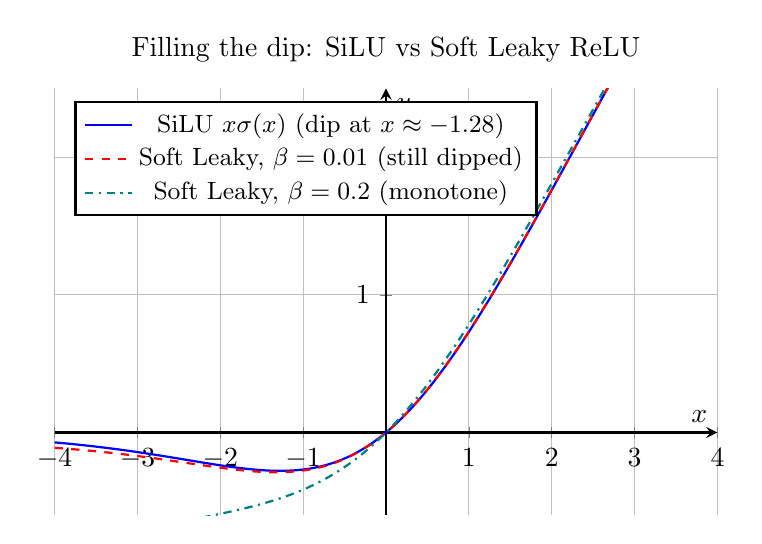
\begin{tikzpicture}
\begin{axis}[
  width=10cm, height=7cm,
  xlabel=$x$, ylabel=$y$,
  title={Filling the dip: SiLU vs Soft Leaky ReLU},
  xmin=-4, xmax=4, ymin=-0.6, ymax=2.5,
  axis x line=middle, axis y line=middle,
  grid=major, legend pos=north west,
  legend style={font=\small},
  samples=300, thick,
]
% SiLU: x * sigmoid(x)
\addplot[blue] {x/(1+exp(-x))};
\addlegendentry{SiLU $x\sigma(x)$ (dip at $x\approx-1.28$)}
% Soft Leaky ReLU beta=0.01
\addplot[red, dashed] {0.99*x/(1+exp(-x)) + 0.01*x};
\addlegendentry{Soft Leaky, $\beta=0.01$ (still dipped)}
% Soft Leaky ReLU beta=0.2 (monotone)
\addplot[teal, dashdotted] {0.8*x/(1+exp(-x)) + 0.2*x};
\addlegendentry{Soft Leaky, $\beta=0.2$ (monotone)}
\end{axis}
\end{tikzpicture}
\end{document}
